\RequirePackage{luatex85}
\documentclass[border=1pt]{standalone}
\usepackage{tikz}
\usetikzlibrary{positioning, shapes.geometric, arrows}

%%%%%%%%%%%%%%%%%%%%%%%%%%%%%%%%%%%%%%%%%%%%%%%%%%%%%%%%%%%%%%%%%%%%%%%%%%%%%%%%
%%%%%%%%%%%%%%%%%%%%                 colours                %%%%%%%%%%%%%%%%%%%% 
%%%%%%%%%%%%%%%%%%%%%%%%%%%%%%%%%%%%%%%%%%%%%%%%%%%%%%%%%%%%%%%%%%%%%%%%%%%%%%%%

\definecolor{tugreen}{RGB}{128, 186, 38}
\definecolor{tucitron}{RGB}{249, 219, 0}



%%%%%%%%%%%%%%%%%%%%%%%%%%%%%%%%%%%%%%%%%%%%%%%%%%%%%%%%%%%%%%%%%%%%%%%%%%%%%%%%
%%%%%%%%%%%%%%%%%%%%                 Boxes                  %%%%%%%%%%%%%%%%%%%% 
%%%%%%%%%%%%%%%%%%%%%%%%%%%%%%%%%%%%%%%%%%%%%%%%%%%%%%%%%%%%%%%%%%%%%%%%%%%%%%%%
\tikzstyle{normalBox} = [shape=rectangle, draw=black, text=black, thick, 	
	align=center, fill=white]

\tikzstyle{roundBox} = [shape=circle, draw=black, text=black, thick, 	
	align=center, fill=white]

\tikzstyle{alternBox} = [shape=rectangle, text=white, thick, align=center, 
	fill=black, rounded corners]


%%%%%%%%%%%%%%%%%%%%%%%%%%%%%%%%%%%%%%%%%%%%%%%%%%%%%%%%%%%%%%%%%%%%%%%%%%%%%%%%
%%%%%%%%%%%%%%%%%%%%                 Arrows                 %%%%%%%%%%%%%%%%%%%% 
%%%%%%%%%%%%%%%%%%%%%%%%%%%%%%%%%%%%%%%%%%%%%%%%%%%%%%%%%%%%%%%%%%%%%%%%%%%%%%%%

\tikzstyle{normalArrow} = [thick,->,>=stealth, draw=black]

\usepackage[utf8]{inputenc}
\usepackage[T1]{fontenc}
\usepackage[sfdefault]{FiraSans}


\tikzstyle{NormalBox} = [normalBox, text width =2.5cm, minimum height=1cm]
\tikzstyle{AlternBox} = [alternBox, text width =2.5cm, minimum height=1cm]

\begin{document}
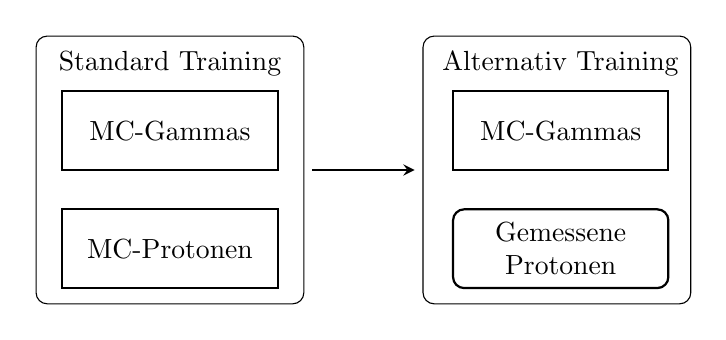
\begin{tikzpicture}[node distance=1.5cm]
  \draw[black, opacity=0] (-1.8,1.8) rectangle (6.7,-1.8); %, opacity=0
  \node (rect) at (0,0) [draw=black,rounded corners ,minimum width=3.4cm,minimum height=3.4cm] {};
  \node (text) at (0,1.35) [text=black] {Standard Training};
  \node (MCGAM) at (0,0.5) [NormalBox] {MC-Gammas};
  \node (MCPRO) [NormalBox, below of=MCGAM] {MC-Protonen};


  \node (rect2) [right=of rect, draw=black,rounded corners ,minimum width=3.4cm,minimum height=3.4cm] {};
  \node (text2) [right=of text, text=black, xshift=0.3cm] {Alternativ Training};
  \node (MSGAM) [right=of MCGAM, NormalBox, xshift=0.7cm] {MC-Gammas};
  \node (MCPRO2) [right=of MCPRO, NormalBox,rounded corners, xshift=0.7cm] {Gemessene Protonen};

  \draw [normalArrow, shorten <=0.1cm,shorten >=0.1cm] (rect) -- (rect2);
\end{tikzpicture}
\end{document}
